\documentclass{sigchi}

% Use this command to override the default ACM copyright statement (e.g. for preprints). 
% Consult the conference website for the camera-ready copyright statement.


%% EXAMPLE BEGIN -- HOW TO OVERRIDE THE DEFAULT COPYRIGHT STRIP -- (July 22, 2013 - Paul Baumann)
% \toappear{Permission to make digital or hard copies of all or part of this work for personal or classroom use is 	granted without fee provided that copies are not made or distributed for profit or commercial advantage and that copies bear this notice and the full citation on the first page. Copyrights for components of this work owned by others than ACM must be honored. Abstracting with credit is permitted. To copy otherwise, or republish, to post on servers or to redistribute to lists, requires prior specific permission and/or a fee. Request permissions from permissions@acm.org. \\
% {\emph{CHI'14}}, April 26--May 1, 2014, Toronto, Canada. \\
% Copyright \copyright~2014 ACM ISBN/14/04...\$15.00. \\
% DOI string from ACM form confirmation}
%% EXAMPLE END -- HOW TO OVERRIDE THE DEFAULT COPYRIGHT STRIP -- (July 22, 2013 - Paul Baumann)


% Arabic page numbers for submission. 
% Remove this line to eliminate page numbers for the camera ready copy
% \pagenumbering{arabic}


% Load basic packages
\usepackage{balance}  % to better equalize the last page
\usepackage{graphics} % for EPS, load graphicx instead
\usepackage{times}    % comment if you want LaTeX's default font
\usepackage{url}      % llt: nicely formatted URLs

% llt: Define a global style for URLs, rather that the default one
\makeatletter
\def\url@leostyle{%
  \@ifundefined{selectfont}{\def\UrlFont{\sf}}{\def\UrlFont{\small\bf\ttfamily}}}
\makeatother
\urlstyle{leo}


% To make various LaTeX processors do the right thing with page size.
\def\pprw{8.5in}
\def\pprh{11in}
\special{papersize=\pprw,\pprh}
\setlength{\paperwidth}{\pprw}
\setlength{\paperheight}{\pprh}
\setlength{\pdfpagewidth}{\pprw}
\setlength{\pdfpageheight}{\pprh}

% Make sure hyperref comes last of your loaded packages, 
% to give it a fighting chance of not being over-written, 
% since its job is to redefine many LaTeX commands.
\usepackage[pdftex]{hyperref}
\hypersetup{
pdftitle={Who to Blame? Understanding Distribution of Responsibility in Human-Robot Interaction},
pdfauthor={LaTeX},
pdfkeywords={SIGCHI, proceedings, archival format},
bookmarksnumbered,
pdfstartview={FitH},
colorlinks,
citecolor=black,
filecolor=black,
linkcolor=black,
urlcolor=black,
breaklinks=true,
}

% create a shortcut to typeset table headings
\newcommand\tabhead[1]{\small\textbf{#1}}


% End of preamble. Here it comes the document.
\begin{document}

\title{Who to Blame?\\ Understanding Distribution of Responsibility in Human-Robot Interaction}

\numberofauthors{3}
\author{
  \alignauthor  Stephen Gaschignard\\
    \affaddr{Department of Computer Sciences}\\
    \affaddr{UW-Madison}\\
    \email{gaschignard@wisc.edu}\\
  \alignauthor Mert Oguz\\
    \affaddr{Department of Computer Sciences}\\
    \affaddr{UW-Madison}\\
    \email{moguz@wisc.edu}\\    
  \alignauthor Xiang Zhi Tan\\
    \affaddr{Department of Computer Sciences}\\
    \affaddr{UW-Madison}\\
    \email{xtan28@wisc.edu}\\
}

\maketitle

\begin{abstract}
Robotic products are not perfect and are prone to make mistakes. This study aims to understand how people attribute blame to different stakeholders when mistakes occur. We hypothesized that both the type and severity will influence how participants distribute blame between the stakeholders in the different situations. We categorized the mistakes into psychological, physical and financial and separated them further by severity. Our first hypothesis states that the robot will receive more responsibility for psychological mistakes. Our second hypothesis states that the robot will receive more responsibility for less severe mistakes. We conducted a within-subject study where 49 participants watched six video scenarios with a robot making a mistake and attributed responsibility to each stakeholder. We found no evidence to support our hypotheses. The evidence indicated that the type of mistakes influenced the amount of blame, where severity of mistakes have no effect. Our study did indicate a greater level of understanding of how machines and robots work by the general population.
\end{abstract}

\section{Introduction}

With the enhancement of robotics and artificial intelligence studies, robots have entered our lives in numerous ways. From industrial robots used in factories to everyday electronics like cleaning robots, humans take advantage of the cutting-edge technology that is designed for them. While studies about robotics deal with development and optimization of such technologies, the scope of human robot interaction studies expands through understanding psychological processes which humans come across while interacting with robots. Many notions which are vastly studied for human-human interaction such as trust, harm and perception of mistakes have been extended into human-robot interaction. \cite{freedy2007measurement}. It is clear that robots make mistakes during the interaction, therefore the performance of the robot is one of the most important reasons for trust to diminish. \cite{hancock2011meta}. Whether the other body is a human or robot, people tend to trust if there is consistency in the behavior of the other. Making mistakes on the other hand, is a natural outcome of poor analysis of the enclosing environment, sometimes caused by different deficiencies. Humans have a high try and fail learning capability, besides many creative mistake recovery strategies. With today's technology, robots are still not as talented as humans in terms of communication with other humans or direct interaction. Therefore, in the upcoming years, we predict that a number of studies will be conducted about the robot-made mistakes. As it is interesting to study why robots make mistake, studying how people perceive those mistakes and how they react in such situations is also crucial for designing successful mistake recovery systems.

Our research question focuses on the human perception of the possible robot mistakes in a restaurant setting. We have decided on this setting since we believe that robot waiters might be conventional in the near future. Restaurants are the places where at least a number of interactions occur between the customer and the waiter. These interactions include physical ones where the waiter brings the menu, dish or the bill. Conventionally, a waiter talks to a customer for getting the order or accepting the payment. These interactions have a psychological effect on the customer. Many customers decide on the amount of tip they wish to give based on the behavior of the waiter. Therefore, we categorized the interactions into different types to be studied.  We analyzed 3 different types of mistakes with 2 different severity levels. Our research is a within-participant study conducted with 49 participants (26 of them were females) where each participant is a U.S. resident. We hired participants through Amazon Mechanical Turk, paying them for completing our online questionnaire. 

In order to reach a more random participant population, we used video-based research instead of lab-based live settings. \cite{woods2006comparing} showed that video-based methods have reasonable results for new innovative studies. This approach enabled us to conduct our study with much smaller budget and time spending. Instead, we could focus on the scenarios and the quality of the questionnaire. 6 scenarios (3 types of mistakes: Physical, Psychological, Financial and 2 severity levels: Severe, Non severe) are designed for the study. After watching every video scenario, we asked participants how they attribute responsibility to each of the stakeholders (The robot, programmer of the robot, owner of the restaurant, manager of the restaurant, manufacturer). Then, we asked them what would be their reaction in such situations. We hypothesized that both the type and severity of the mistake will influence participants' distribution of blame. We further predicted that people will blame the robot more for psychological abuse. Our last hypothesis was people will blame the robot for non-severe situations, whereas they will blame other stakeholders for severe situations, if the mistake is a financial exploitation or physical abuse.

\section{Methodology}
\subsection{Research Question}
How do different types of errors in human-robot interaction affect the human’s perception on distribution of culpability?

\subsection{Hypotheses}
\textit{Hypothesis 1:} The participants will blame the robot regardless of the severity of the error if the error is a psychological abuse.

In the case of psychological harm, people tend to react immediately to the body who caused the harm. On the other hand, it is shown that the people attribute a higher level of accountability to a robot than an ordinary computer system.

\textit{Hypothesis 2:} For the scenarios where the error is a financial exploitation or physical abuse, the participants will blame the robot for non-severe situations; whereas they will blame other stakeholders for severe situations.

The severe errors of physical or financial harm usually have long-term effects which causes people to blame the company or person that is responsible for the operation/ production of the robots. For instance when a plane accident occurs, people tend to blame the airline company even if the problem is caused by a rare mechanical malfunction. On the other hand, non-severe problems don’t require people to look for other stakeholders other than the robot itself.

\subsection{Experimental Design}
We used a 3 (type of mistake) x 2 (severity of mistake)  within-participants experimental design for this research study. Each participant viewed videos showing different scenarios with human-robot interactions - the videos represented each type and severity of harm that we were modifying to measure the effects of these factors.

\subsection{Experimental Task}
Each participant was introduced to a robot restaurant waiter through a video. After becoming familiar with the robot, the participant viewed a series of videos where the robot waiter harmed a human customer at the restaurant in some way. Each video represented each level of the factors described above:
\begin{enumerate}
\item Psychological Abuse
\begin{itemize}
\item Non-severe: robot offered a curry dish to someone who had declared a dislike of curry.
\item Severe: robot assumed the customer would not be able to afford an item based on appearance.
\end{itemize}

\begin{figure}[!h]
\centering
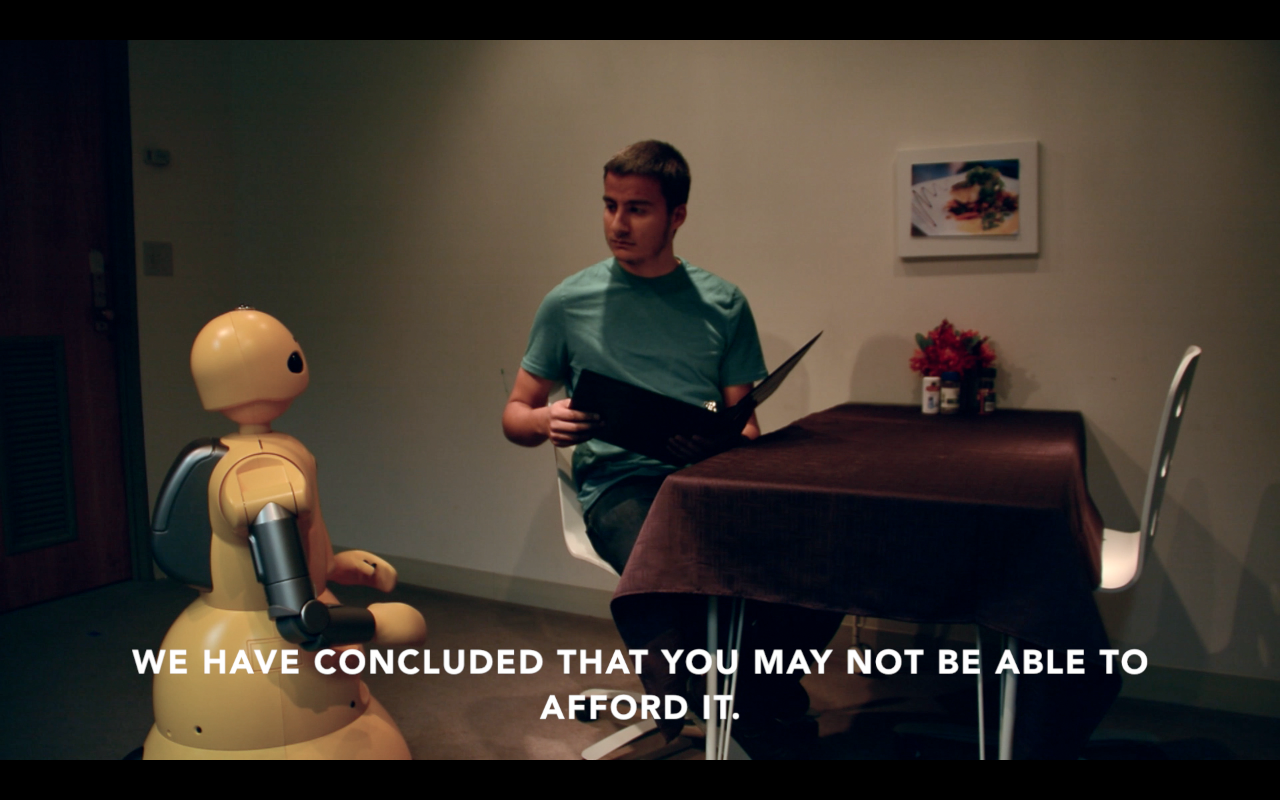
\includegraphics[width=0.8\columnwidth]{Psych-Severe}
\caption{Psychological Harm - More Severe}
\label{fig:figure1}
\end{figure}

\item Financial Exploitation
\begin{itemize}
\item Non-severe: robot neglected to return change to the customer for the meal payment.
\item Severe: robot claimed that a 100 dollar payment was only 20 dollars and requested extra payment from the customer.
\end{itemize}

\begin{figure}[!h]
\centering
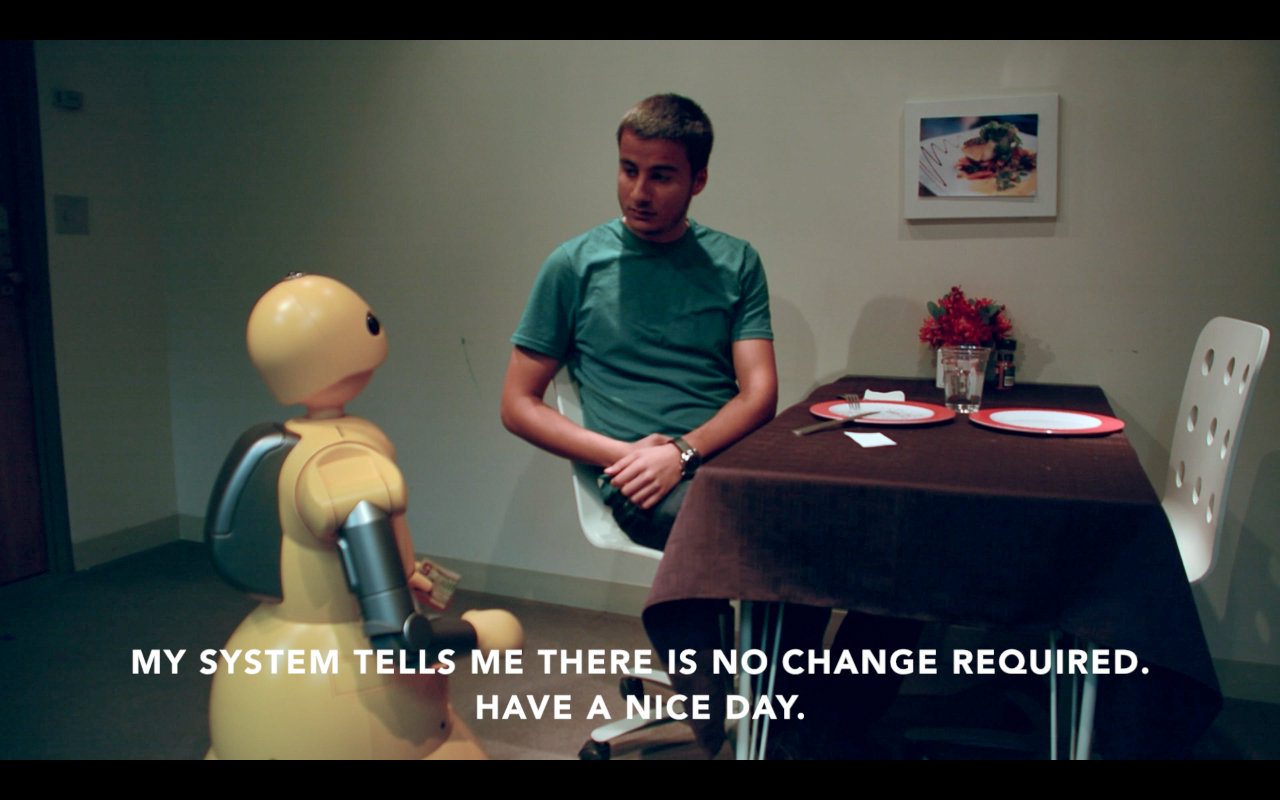
\includegraphics[width=0.8\columnwidth]{Fin-Less}
\caption{Financial Harm - Less Severe}
\label{fig:figure2}
\end{figure}

\item Physical Abuse
\begin{itemize}
\item Non-severe: robot dropped a small silverware item on the customer.
\item Severe: robot dropped a hot food dish on the customer.
\end{itemize}

\begin{figure}[!h]
\centering
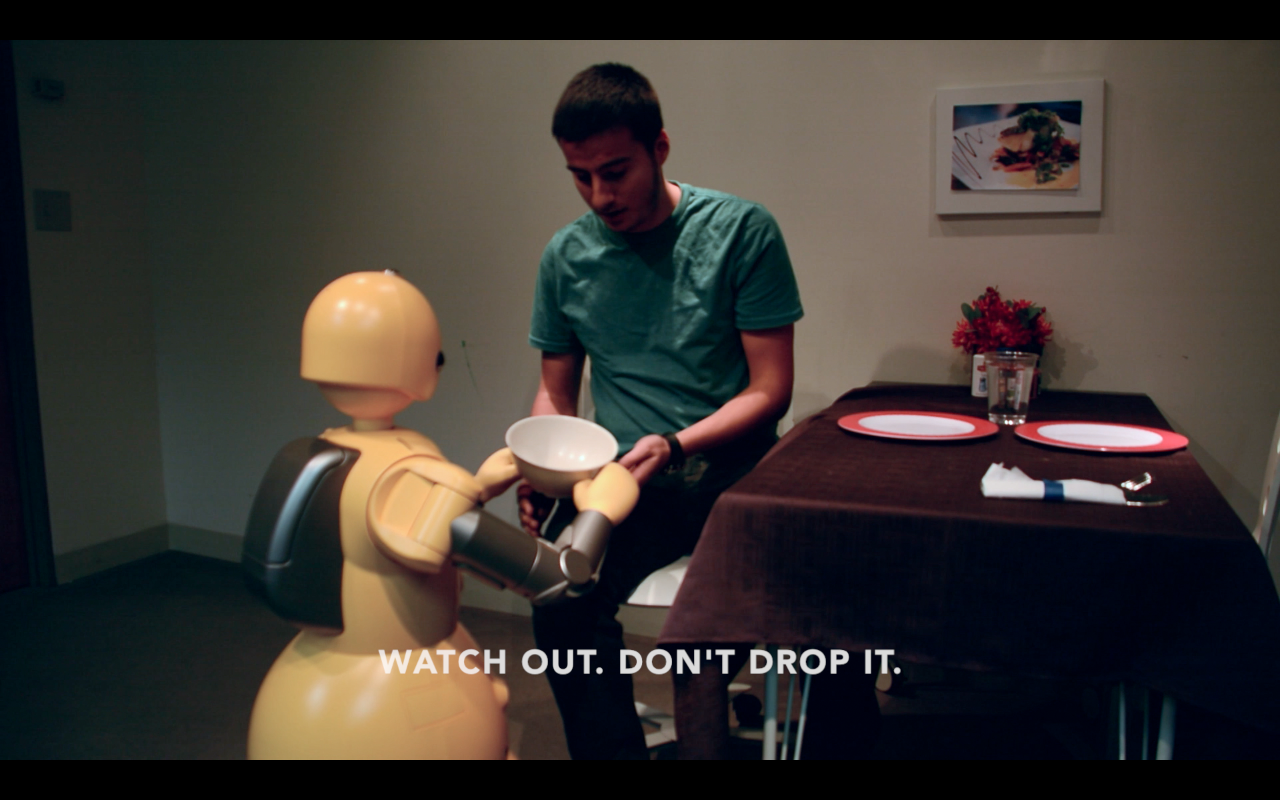
\includegraphics[width=0.8\columnwidth]{Phys-Severe}
\caption{Physical Harm - More Severe}
\label{fig:figure3}
\end{figure}

\end{enumerate}

Each video was as realistic as possible - we used a real robot in the videos. We encouraged the participants to imagine that they were the human customer that was harmed in each video in order to elicit the most accurate reaction and perception of each events.

\subsection{Experimental Procedure}
The study was conducted over the internet where participants were asked to logged on to private website. After consenting to the survey, the participant was introduced to the robot via a descriptive graphic. This graphic showcased the intelligence and advance features in the robot. Afterwards, the participant was assigned each video in random order. In each mistake type, participant was randomly assign a severity condition and shown the video of mistake type with that severity condition. After finishing the video, the participant was asked to complete a questionnaire about their perception towards the robot in the video. Upon completing all the conditions, the participant filled up a final questionnaires about demographic data. Once the participant finished the questionnaire, the participant was given between 0.35 and 0.50 dollars as compensation for their participation.

\begin{figure}[!h]
\centering
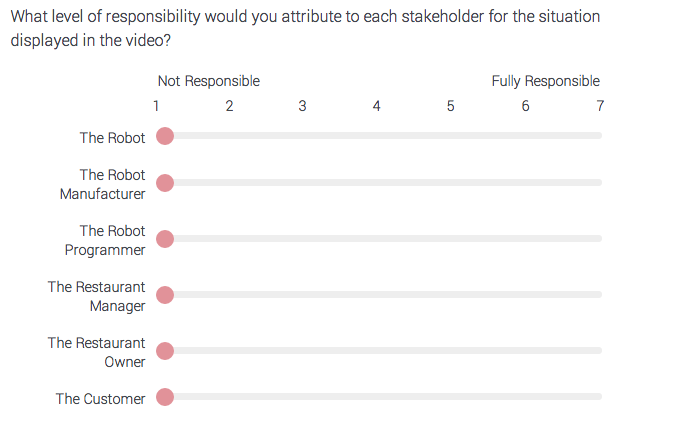
\includegraphics[width=0.9\columnwidth]{Survey}
\caption{Screenshot of survey question with Likert scale}
\label{fig:figure4}
\end{figure}

\subsection{Measurements}
In each condition, participants were asked to identify the possible parties responsible for the mistake in the questionnaire . The participants were given a list of parties involve such as the robot, manager on duty, company that owns the robot, programming team for the robot, the manufacturer of the robot, or the customer. In the list, participants were able to rank the parties they believed were responsible for the incident. When identifying each stakeholder, the particiapnt was asked to give a rating of the stakeholder's culpability using a 1-7 likert scale. If the participant believe there were no parties to be blamed, the participant could refrain from attributing blame to any stakeholder. 

To validate the successful manipulation of the independent variables, participants were also asked to rank the severity of each mistake on a 1-7 likert scale, where 1 is least severe and 7 as most severe. As the study was conducted through a web portal, we asked a validation question ("How much money was given to the robot in the previous video?") to ensure participants were following the procedure of the study.

\subsection{Participants}
50 participants (24 male and 26 female) were recruited through the Amazon mTruck Infrastructure and social media platform. One male participant's responses were removed from the data due to a failure to correctly respond to one of our data response validity questions. The participants were limited to people living in  United States.

\section{Findings}
\subsection{Manipulation Check}
We conducted a manipulation check to verify the success of manipulation in our condition. After watching each video clip, we asked participants to rate the severity for each scenario. We found in all scenarios, that the participants rated the severe condition significantly higher than the non-severe condition.

\begin{table}
  \centering
  \begin{tabular}{|c|c|c|c|}
    \hline
    Type & Non-Severe & Severe & p Value \\
    \hline
    Financial & 3.633 & 4.918 & 0.0003 \\
    \hline
    Psychological & 2.633 & 5.020 & $ < 0.0001$ \\
    \hline
    Psychological & 2.816 & 5.020 & $ < 0.0001$ \\
    \hline
  \end{tabular}
  \caption{Mean difference between perceive severity}
  \label{tab:table1}
\end{table}

\subsection{Result}
To test our hypotheses, we carried analysis of variance (ANOVA) on the collected result. 

In our first hypothesis, we claimed that robots will be blamed significantly more than other stakeholders in the psychological harm condition. To verify the hypothesis, we ran a one-way ANOVA on the result and found no evidence to support our hypothesis. We found that the participants blamed programmer most (mean = 6.28), comparing to other stakeholders. In relation to our hypothesis, participants blamed programmer ($ F(1,582) =139.1, p < .0001$), owner ($ F(1,582) = 19.68, p < .0001$), manufacturer ($F(1,582) = 38.28, p < .0001$) and manager ($F(1,582) = 13.38, p = 0.0003$) more than the robot. Customer was the only stakeholder which has been blamed significantly less than the robot ($F(1,582) = 54.09, p < .0001$).

\begin{table}[h]
  \centering
  \begin{tabular}{|c|c|c|}
    \hline
    Stakeholders & Mean & Standard Deviation\\
    \hline
    Robot & 3.184 & 0\\
    \hline
    Customer & 1.255 & 0\\
    \hline
    Manager & 4.142 & 0 \\
    \hline
    Manufacturer & 4.806 & 0 \\
    \hline
    Owner & 4.34694 & 0 \\
    \hline
    Programmer & 6.286 & 0 \\
    \hline
  \end{tabular}
  \caption{Mean Difference between perceive severity}
  \label{tab:table2}
\end{table}

Our second hypothesis states that participants would blame robots for less severe mistakes in financial and physical harm but will blame other stakeholders for severe mistake. We ran a two-way ANOVA on our result and found no result that supports our hypothesis.


We found the severity of the condition significantly influence participants blame on the robot($F(1,240), p = 0.0159$). However the difference between conditions was only 0.22. The type of the condition also affected the blame on robot($F(2,240)=9.280, p = 0.0001$). Participants blame the robot less in psychological condition compare to Physical($F(1,240)=18.27, p < .0001$) and financial($F(1,240)=6.77, p = 0.0098$). No interaction effect was found between severity and type of mistake.

We also found that severity of the condition has a significant effect on the rate of blame for manufacturers($F(1,240)=7.4947, p = 0.0067$). We see a small increase of 0.35 from non-severe to severe. The blaming of manufacturers are also influence by the type of condition($F(2,240)=7.4736, p=0.0007$). In doing pairwise analysis, we found that manufacturers are blamed less for financial($F(1,240)=5.828, p = 0.0165$) and physical($F(1,240)=14.610, p = 0.0002$).

When asked about the responsibility of the programmers in these mistakes, the type of mistake influence the distribution of blame($F(2,240)=12.577, p < .0001$). Participants blame the programmers more for both the financial condition($F(1,240)=15.214, p < 0.0001$) and psychological condition($F(1,240)=21.91, p < 0.0001$).

We also saw a small significant effect of type of mistake in blaming the manager for the mistake of the robot($P(1,240)=11.31, p = 0.0009$). Participants were shown to increase the blame of the manager when the mistake was more severe. We also saw an interaction effect between Severity and Type for the manager($F(2,240)=3.7958, p = 0.0238$)

For owners, we saw there was a significant effect of the severity of the condition on the blaming of owners($F(1,240)=12.02, p=0.0006$). We also saw interaction effect between severity and type of condition on the blaming of owner.

We did not found any effects of severity and interaction effect for the blaming of customer. However, we observe that the type of mistake significantly effect the assignment of blame($F(2,240)=9.19, p=0.0001$).In pair wise analysis, we found participants blame the robot more in the physical condition compare to the financial($F(1,240)=7.2609, p = 0.0075$) and psychological condition($F(1,240)=17.9301, p < .0001$)

\section{Discussion}
Returning to our hypotheses, we were looking for our results to show that the participants would blame the robot more in situations involving psychological harm, and for the results to show more blame for other stakeholders in more severe situations. However, our results did not contribute to our hypotheses in any way. Based on the analysis of our data, there is no significant difference in how much the participants blame the robot for psychological harm versus other types of harm. In addition to that, severity appears to have no effect on the distribution of blame whatsoever.

We did find that in all cases (between each level of severity and type of harm), the programmer consistently took the highest amount of blame. This is interesting because it alludes to a higher level of understanding of how robot's work by the everyday person in the United States. At the basis of our study, we assumed that most participants would see robots as independent beings with their own independent actions. The high level of blame attributed to the programmer implies that the everyday person understands that robots do not have their own free will, but that they are acting as instructed by those who programmed them.

The data analysis also displayed a significant increase in the level of blame attributed to the customer in scenarios with physical harm compared to psychological or financial harm. We see this as a result of our survey design and not necessarily as a result that can or should be applied to all scenarios with physical harm. In the two video scenarios that we use, the robot dropped an object (either silverware or a hot bowl) while handing over the object to the customer. It may have been possible for the customer to prevent the situation by catching the object before it fell, which may have been a reason to attribute more blame to the customer. Although the result is statistically significant, we do not see it as a result that is applicable outside of the context of our study.

In terms of severity, we found that there was an increase in the total amount of blame that was attributed to each stakeholder for the more severe situations. There was no relative increase in the amount of blame one stakeholder received over another - instead, the level of blame attributed to each individual stakeholder across the board saw a significant increase for more severe situations over less severe situations. 

There is another component of the survey design that may have influenced our results. When asking the participants to allocate blame between different stakeholders, we listed six different stakeholders for the participant to choose from. We believe this influenced the participant to read through and fully consider each of the listed stakeholders instead of writing down who they instinctively blamed from their initial reaction to the scenarios. We may have seen a different distribution of blame between stakeholders using this approach compared to the data we collected.

\section{Conclusion}
Despite our initial hypotheses, a human would not attribute more blame to a robot for psychological harm or for less-severe mistakes. However, our results did indicate that there is a better understanding of robots by the general US population: we saw that people comprehend that robots are acting as instructed by programmers and not out of their own independent free will, and as such people will tend to blame programmers for a robot's mistakes.

\section{References format}
References must be the same font size as other body text.
% REFERENCES FORMAT
% References must be the same font size as other body text.
\bibliographystyle{acm-sigchi}
\bibliography{reference}
\end{document}
